\section{Introduction}
\label{sec:introduction}

Cooperative Multi-Agent Reinforcement Learning (MARL) has achieved remarkable empirical breakthroughs across symmetric coordination tasks, most notably in the StarCraft Multi-Agent Challenge (SMAC)~\cite{yu2022surprising,rashid2020monotonic} and cooperative swarm robotics. In these domains, agents typically share homogeneous action sets, symmetric observation fields, and interchangeable tactical objectives. However, a wide spectrum of critical real-world applications---including search-and-rescue operations, multi-robot automated warehouse logistics, and tactical cybersecurity intrusion response---demands \emph{heterogeneous specialization}: agents possess strictly asymmetric sensory capabilities, distinct operational mechanics, and non-interchangeable functional responsibilities.

Under asymmetric role allocations, standard Centralized Training with Decentralized Execution (CTDE) methods~\cite{schulman2017proximal,foerster2018counterfactual} encounter three fundamental bottlenecks:
\begin{enumerate}[leftmargin=*,nosep]
    \item \textbf{Monolithic Representation Collapse:} Shared-parameter networks fail to preserve sharp, role-specific policies when reward signals for distinct sub-tasks---such as stealth navigation, lockpicking, sentry neutralization, or high-value payload transport---arrive at vastly differing temporal frequencies and reward densities.
    \item \textbf{The ``Rich-Get-Richer'' MoE Trap:} Unconstrained value-bidding Mixture-of-Experts (MoE) models~\cite{shazeer2017outrageously,fedus2022switch} frequently collapse into a single monopoly expert. An incumbent generalist with an established high-value critic baseline wins all routing decisions, starving newly spawned or auxiliary specialists of exploratory transitions and gradient updates.
    \item \textbf{Cold-Start Critic Fragility:} Introducing a new specialist to address an empirical failure manifold is futile when its uncalibrated value network cannot submit competitive bids against mature generalists in unconstrained routing tournaments, causing immediate regression.
\end{enumerate}

\begin{figure}[t]
\centering
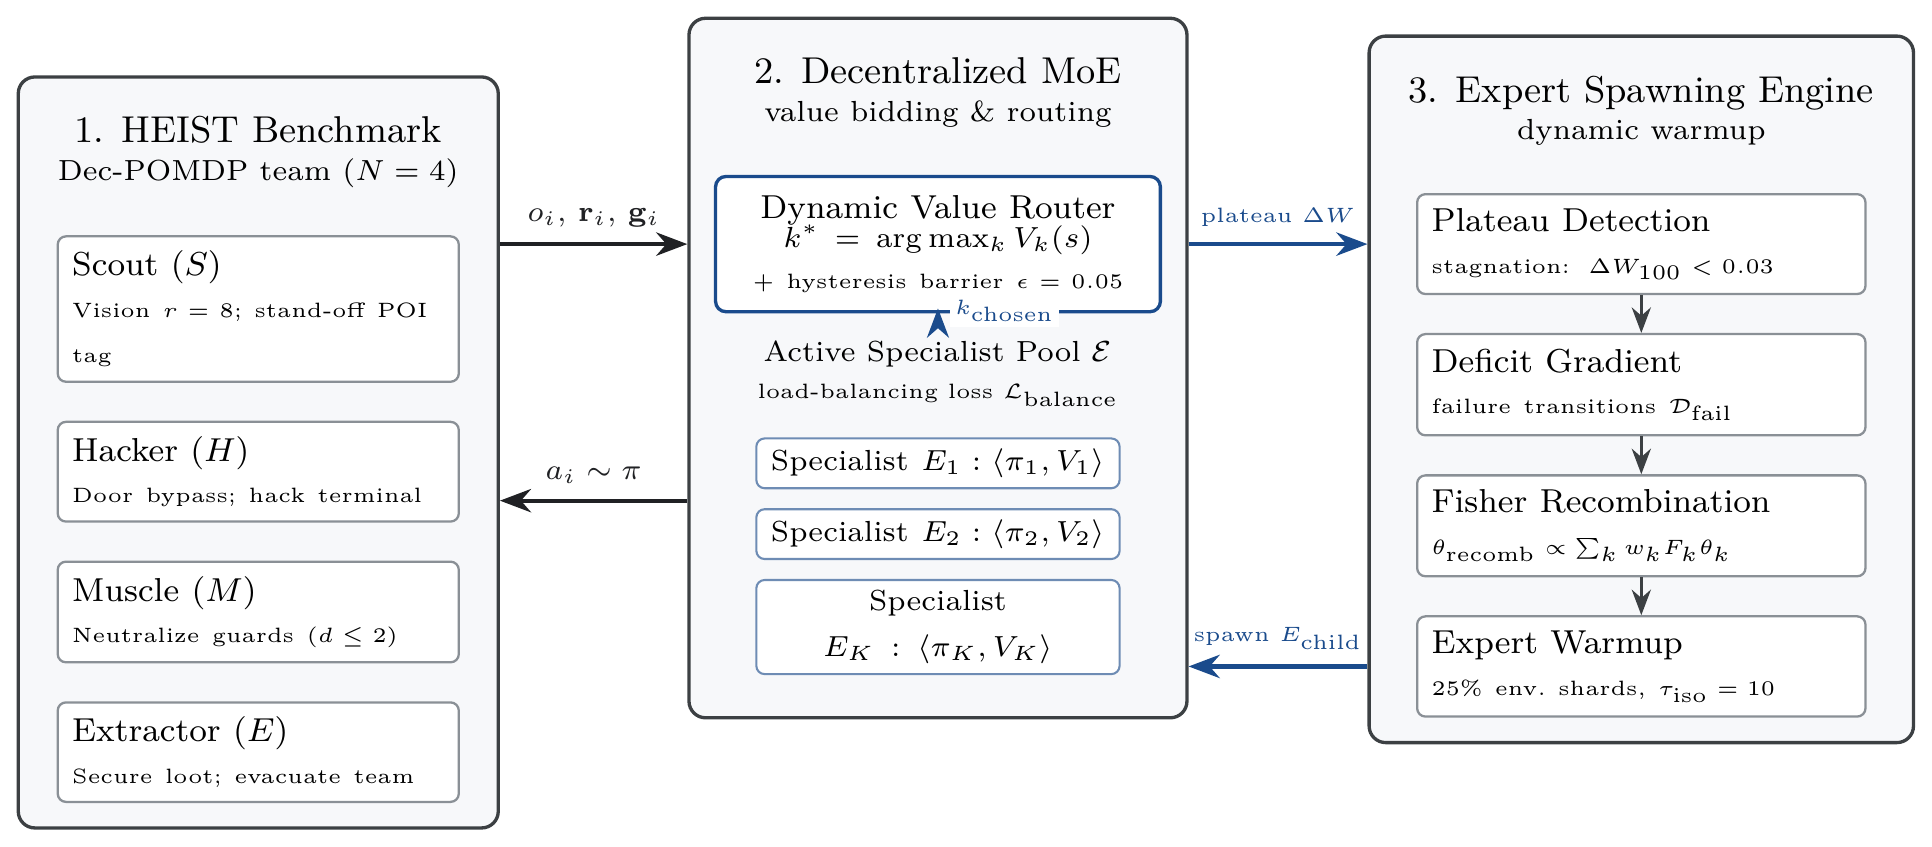
\includegraphics[width=\linewidth]{figures/architecture.pdf}
\caption{\textbf{THIEF Framework Overview.} An open-ended evolutionary Mixture-of-Experts architecture featuring win-rate plateau triggering, failure sub-manifold isolation, Fisher Information parameter recombination, isolated sandbox incubation, and hysteresis-bounded routing with load-balancing regularization.}
\label{fig:architecture}
\end{figure}

To resolve these pathologies, we present an evolutionary architectural progression developed across four iterative generations, culminating in our proposed framework:
\begin{enumerate}[leftmargin=*,nosep]
    \item \textbf{MARC (Multi-Agent Reward Credit):} Our first iteration augments monolithic CTDE with affordance-aware potential-based reward shaping to alleviate spatial credit assignment bottlenecks.
    \item \textbf{COOP (Cooperative MoE):} Our second iteration introduces capacity modularization via a static 2-expert value-bidding pool, demonstrating the necessity of specialized sub-networks but suffering from unconstrained monopoly collapse.
    \item \textbf{E-COOP (Evolutionary Cooperative PPO):} Our third iteration and primary architectural ablation introduces periodic Fisher-weighted parameter recombination into a single champion network ($K=1$). While highly sample-efficient, its critic-cloning mechanism aggressively cannibalizes specialized sub-manifolds.
    \item \textbf{THIEF (Targeted Hysteresis-routed Incubated Evolution via Fisher-geometry):} Our complete framework, combining plateau-triggered expert spawning, failure-directed deficit mutation, all-pool Fisher Information Matrix (FIM) recombination, isolated sandbox incubation on dedicated environment shards, and sparse load-balancing regularization with dormancy freezing.
\end{enumerate}

We introduce the open-source \textbf{HEIST Benchmark} (implemented as a native multi-threaded Rust engine sustaining approximately $12,\!000$ environment steps per second) and evaluate our iterative method lineage against standard external MARL baselines (MAPPO~\cite{yu2022surprising}, H-MAPPO~\cite{vezhnevets2017feudal}, and COMA~\cite{foerster2018counterfactual}) across a 5-stage spatial curriculum ($11 \times 11$ to $50 \times 50$).

In summary, this paper makes the following contributions:
\begin{enumerate}[leftmargin=*,nosep]
    \item \textbf{HEIST Benchmark:} an open-source, high-throughput heterogeneous cooperative MARL environment with asymmetric role mechanics, dynamic adversarial security, and a five-stage spatial curriculum, engineered in Rust with zero-copy PyTorch integration for GPU-accelerated training.
    \item \textbf{THIEF:} an open-ended evolutionary Mixture-of-Experts algorithm that triggers specialist spawning on empirically detected win-rate plateaus, recombines the full specialist pool under Fisher Information geometry, incubates cold-started children on dedicated environment shards, and prevents routing monopoly via hysteresis-bounded bidding and load-balancing regularization.
    \item \textbf{A systematic method lineage as macro-ablation:} MARC, COOP, and E-COOP isolate, in controlled succession, the contributions of credit shaping, modular capacity, and evolutionary recombination, and are benchmarked against external baselines (MAPPO, H-MAPPO, COMA) over $3,\!000$ evaluation episodes per stage.
\end{enumerate}
